\documentclass[11pt,a4paper]{article}
\usepackage[utf8]{inputenc}
\usepackage[T1]{fontenc}
\IfFileExists{lmodern.sty}{\usepackage{lmodern}}{}
\usepackage{amsmath,amssymb,amsthm,bm}
\usepackage{booktabs}
\usepackage{graphicx}
\usepackage[margin=2.5cm]{geometry}
\usepackage{hyperref}
\usepackage{listings}
\usepackage{xcolor}

\lstset{basicstyle=\ttfamily\small,columns=fullflexible,frame=single,
        backgroundcolor=\color{gray!6},breaklines=true,
        literate={Γ}{{$\Gamma$}}1 {θ}{{$\theta$}}1 {Θ}{{$\Theta$}}1 {π}{{$\pi$}}1 {ρ}{{$\rho$}}1}

\setlength{\emergencystretch}{3em}
\newtheorem{proposition}{Proposition}
\newtheorem{remark}{Remark}
\newcommand{\avg}[1]{\{\!\{#1\}\!\}}
\newcommand{\jump}[1]{[\![#1]\!]}
\newcommand{\qh}{\hat{\bm q}}
\newcommand{\q}{\bm q}
\newcommand{\thb}{\bar\theta}
\newcommand{\pib}{\bar\pi}
\newcommand{\D}{\bm D}

\title{The fast linear operator of the Euler equations in\\
potential-temperature form: energy-stable hybridized DGSEM\\
with LMARS flux and relaxed trace conditions}
\author{Documentation of \texttt{hdg\_relax\_theta.py} / \texttt{HDGRelaxTheta.jl}}
\date{\today}

\begin{document}
\maketitle

\begin{abstract}
We derive and discretize the linear fast operator of the one-dimensional (vertical)
compressible Euler equations in the variables $(\rho,\rho w,\rho\theta)$, intended as the fast
(acoustic) part of a split-explicit method. Momentum advection is removed, $\theta$ is frozen in
the $\rho\theta$ equation, and the pressure is written as $p=\frac{p}{\rho\theta}\,\rho\theta$
with $\frac{p}{\rho\theta}$ frozen. The resulting system is linear in the full state and has a
local, weighted quadratic energy. It is discretized by a nodal discontinuous Galerkin spectral
element method (DGSEM) on Gauss--Lobatto nodes in hybridized form. A split form of the volume
terms, built on the summation-by-parts (SBP) property, reproduces the weighted energy identity
exactly. The trace stabilization $\bm T=|\bm A|$ yields the LMARS flux, which is shown to be
energy dissipative. The resulting semi-discretization is provably energy stable, conservative in
$\rho$ and $\rho\theta$, and well balanced. The plain collocation form, by contrast, has a
spurious $\mathcal O(h)$ growth rate. The trace conditions are relaxed into evolution equations,
and the coupled system is integrated without static condensation.
\end{abstract}

\tableofcontents

%=====================================================================
\section{Model and linearization}
%=====================================================================
\subsection{Full equations}
In a vertical column with $m=\rho w$ and $\Theta=\rho\theta$,
\begin{equation}
\partial_t\rho + \partial_z m = 0,\qquad
\partial_t m + \partial_z(m w + p) = -\rho g,\qquad
\partial_t\Theta + \partial_z(\theta m) = 0,\qquad
p = p_{00}\Big(\frac{R\,\Theta}{p_{00}}\Big)^{\gamma}.
\end{equation}

\subsection{Linearization (fast operator)}
Given a frozen state (bars), for example the current slow state, the linearization consists of
three steps.
\begin{enumerate}
\item Remove momentum advection: $\partial_z(mw)\to0$.
\item Freeze $\theta$ in the $\Theta$ equation: $\partial_z(\theta m)\to\partial_z(\thb\,m)$.
\item Write $p=\dfrac{p}{\Theta}\,\Theta$ and freeze the ratio: $p\to\pib\,\Theta$ with
      $\pib=\bar p/\bar\Theta=R\bar\Pi$ ($\Pi$ = Exner function).
\end{enumerate}
This gives
\begin{equation}\label{eq:fast}
\boxed{\;
\partial_t\rho+\partial_z m=0,\qquad
\partial_t m+\partial_z(a\,\Theta+b)=-g\rho,\qquad
\partial_t\Theta+\partial_z(\thb\,m)=0,\;}
\end{equation}
with $a=\texttt{pfac}\,\pib$ and $b=(1-\texttt{pfac})\,\bar p$. The default $\texttt{pfac}=1$ is
the linearization above. The system is linear in the \emph{full} state $\q=(\rho,m,\Theta)$. In
flux form, $\partial_t\q+\partial_z(\bm A\q+b\,\bm e_m)=\bm S\q$ with
\begin{equation}
\bm A=\begin{pmatrix}0&1&0\\0&0&a\\0&\thb&0\end{pmatrix},\qquad
\bm S=\begin{pmatrix}0&0&0\\-g&0&0\\0&0&0\end{pmatrix},\qquad
\operatorname{spec}\bm A=\{0,\pm c\},\quad c^2=a\thb .
\end{equation}

\paragraph{Sound speed.} For $\texttt{pfac}=1$, $c^2=\pib\thb=\bar p/\bar\rho=R\bar T$: freezing
$p/\Theta$ gives the isothermal sound speed (287 instead of 340\,m/s at 288\,K). With
$\texttt{pfac}=\gamma$ one obtains the tangent-linear pressure and $c^2=\gamma R\bar T$; this
variant coincides with the classical linearization about a hydrostatic state at rest. The
constant $b$ keeps $p_{\rm lin}(\bar\Theta)=\bar p$.

\subsection{Use in a split-explicit method}
With the full operator $\mathcal N$ and the fast operator $\mathcal L$ frozen at the slow level
$\q^n$, the fast system over the small steps is
$\partial_t\q=\mathcal L(\q)+\bm F_{\rm slow}$ with
$\bm F_{\rm slow}=\mathcal N(\q^n)-\mathcal L(\q^n)$ held constant (e.g.~\cite{wicker2002}). All
time integrators accept \texttt{F\_slow}, and \texttt{tendency(q)} returns $\mathcal L(\q)$.

%=====================================================================
\section{Energy of the frozen system}
%=====================================================================
Let $p=a\Theta$ and let $\chi=\Theta-\thb\rho$ be the $\theta$-perturbation. From
\eqref{eq:fast},
\begin{equation}\label{eq:chi}
\partial_t\chi = -\partial_z(\thb m)+\thb\,\partial_z m = -\thb_z\,m .
\end{equation}
\begin{proposition}[Energy]\label{prop:energy}
Let $\varphi(z)=\thb(z)\exp\!\big(\int^z g/c^2\,dz'\big)$. For deviations from a steady state,
\begin{equation}\label{eq:E}
E=\frac12\int\varphi\Big[m^2+\frac{p^2}{c^2}+\frac{g}{\thb\,\thb_z}\,\chi^2\Big]dz,
\qquad \frac{dE}{dt}=-\big[\varphi\,p\,m\big]_{\partial\Omega}.
\end{equation}
$E$ is positive definite if the frozen stratification is stable ($\thb_z>0$).
\end{proposition}
\begin{proof}
Write $\rho=(\Theta-\chi)/\thb$ in the momentum equation. Testing the momentum equation with
$\varphi m$ and \eqref{eq:chi} with $\varphi g\chi/(\thb\thb_z)$ gives two terms
$\pm\varphi g m\chi/\thb$, which cancel. Testing the $\Theta$ equation with
$\varphi p/c^2=\varphi\Theta/\thb$ and integrating by parts gives
$-[\varphi p m]+\int m\,\partial_z(\varphi p)-\int\varphi p\,\thb_z m/\thb$. Together with the
momentum term $-\int\varphi m(\partial_z p+g\Theta/\thb)$, the remainder is
$\int m\,p\,(\varphi_z-\varphi\thb_z/\thb-\varphi g/c^2)$, which vanishes by the choice of
$\varphi$.
\end{proof}
The energy is local in $(\rho,m,\Theta)$ but \emph{weighted}, and it couples $\rho$ and $\Theta$
through $\chi$. A Galerkin method with unweighted test functions does not reproduce
\eqref{eq:E}. This is the origin of the instability of the standard form (Section~\ref{sec:stab}).

%=====================================================================
\section{Hybridized DGSEM discretization}
%=====================================================================
\subsection{Nodal basis and SBP property}
Each element $K_e$ (size $h$, Jacobian $J=h/2$) carries the Lagrange polynomials on the $p+1$
Gauss--Lobatto--Legendre (GLL) nodes $\xi_i$ with weights $w_i$. The unknowns are nodal values,
and quadrature is collocated at the nodes. The mass matrix is
$\bm M=J\,\bm W=J\operatorname{diag}(w_i)$, and the differentiation matrix
$D_{ij}=\ell_j'(\xi_i)$ satisfies the SBP property~\cite{kopriva,gassner2013}
\begin{equation}
\bm W\D+\D^{\mathsf T}\bm W=\bm B=\operatorname{diag}(-1,0,\dots,0,1).
\end{equation}
Products of the frozen coefficients with the unknowns are evaluated pointwise at the nodes. The
element end nodes coincide with the faces, so the face values are just the end-node values.

\subsection{Split-form volume terms}
At node $i$ (all quantities nodal, $(\D u)_i=\sum_jD_{ij}u_j$):
\begin{align}
\dot\rho_i &= -\tfrac1J(\D m)_i \;+\;\text{SAT},\\
\dot\Theta_i &= -\tfrac1J\big(\thb_i(\D m)_i+m_i(\D\thb)_i\big) \;+\;\text{SAT},\label{eq:Th}\\
\dot m_i &= -\tfrac1J\Big[\tfrac{1}{\varphi_i}\big(\D(\varphi a\Theta)\big)_i
 -\tfrac{a_i\Theta_i}{\thb_i}(\D\thb)_i+(\D b)_i\Big]+\frac{g\,\Theta_i}{\thb_i}-g\rho_i
 \;+\;\text{SAT}.\label{eq:m}
\end{align}
\begin{itemize}
\item The $\Theta$ flux is in product-rule form. By SBP,
$\sum_iw_i[\thb_i(\D m)_i+m_i(\D\thb)_i]=[\thb m]_{-1}^{1}$, so $\Theta$ is still exactly
conserved. Moreover, $\dot\chi_i=-(\D\thb)_i m_i/J$ holds exactly at every node, which is the
discrete version of \eqref{eq:chi}.
\item The pressure gradient \eqref{eq:m} is consistent with $\partial_z(a\Theta+b)$, because
$\varphi^{-1}\partial_z(\varphi p)-p\thb_z/\thb-g\Theta/\thb=\partial_zp$ by the definition of
$\varphi$. It is the form for which the discrete energy identity holds.
\item The nodal values $\varphi_i$ are computed from $\thb$ and an accurate quadrature of
$\int g/c^2$. They are continuous across faces.
\end{itemize}

\subsection{Traces, SAT and the LMARS flux}
Let $b$ be an end node of an element with outward normal $n$, and $f$ its face. The coupling to the
trace is
\begin{equation}
J\,w_b\,\dot{\q}_b \mathrel{+}= (\bm A_fn-\bm T_f)(\q_b-\qh_f),\qquad
\bm T_f=|\bm A_f|=\begin{pmatrix}0&0&a_f/c_f\\0&c_f&0\\0&0&c_f\end{pmatrix}.
\end{equation}
This is the strong-form SAT with the hybridized flux
$\widehat{\bm F}\cdot n=\bm A_f\qh\,n+\bm T_f(\q_b-\qh)$. The trace conditions are
$\qh_f=\avg{\q}$ at interior faces and $\qh_f=\operatorname{diag}(1,0,1)\,\q_{\rm int}$ at walls
($\hat m=0$). With them, the face flux is exactly LMARS~\cite{chen2013}:
\begin{equation}\label{eq:lmars}
m^\ast=\avg m-\frac{\jump{p}}{2c_f},\qquad p^\ast=\avg{p}+b_f-\frac{c_f}{2}\jump m,\qquad
\text{$\Theta$ flux}=\thb_f\,m^\ast ,
\end{equation}
with $p=a\Theta$. Since $c_f^2=a_f\thb_f$, the $\Theta$ flux equals $\thb_f$ times the mass flux.

\begin{proposition}[Discrete energy stability]\label{prop:dstab}
Let $\Delta\q$ be the deviation from a discrete steady state, and let $\thb$ be stably stratified
at the nodes ($(\D\thb)_i>0$). For the split form with LMARS traces and $\varepsilon=0$, the
discrete energy
\[
E_h=\frac12\sum_e J\sum_i w_i\varphi_i\Big[m_i^2+\frac{a_i}{\thb_i}\Theta_i^2+
\frac{g}{\thb_i(\D\thb)_i/J}\chi_i^2\Big]
\]
satisfies
\[
\frac{dE_h}{dt}=-\sum_{\text{interior }f}\varphi_f\Big(\frac{c_f}{2}\jump m^2+\frac{1}{2c_f}\jump p^2\Big)
-\sum_{\text{walls}}\varphi_f\,c_f\,m_b^2\;\le\;0 .
\]
\end{proposition}
\begin{proof}[Sketch]
The proof mirrors Proposition~\ref{prop:energy}, with SBP replacing integration by parts:
\begin{itemize}
\item The $\chi$ terms cancel pointwise, because $\dot\chi_i=-(\D\thb)_im_i/J$ holds exactly.
\item The volume terms reduce to $-[\varphi p m]$ at each element's ends. This uses
$\sum_iw_i\psi_i(\D m)_i=[\psi m]-\sum_iw_im_i(\D\psi)_i$ with $\psi=\varphi a\Theta/\thb$.
\end{itemize}
At each element end, the volume boundary term and the SAT contributions combine to
$-\varphi\,[m\,p^\ast+p\,m^\ast-p\,m]\,n$. The $\chi$ parts of the SAT cancel because the
$\Theta$ flux is $\thb_f$ times the mass flux. Summing the two sides of an interior face and
inserting \eqref{eq:lmars} gives
$\varphi_f(p^\ast\jump m+m^\ast\jump p-\jump{pm})=-\varphi_f(\tfrac{c_f}{2}\jump m^2+\tfrac{1}{2c_f}\jump p^2)$.
At walls, $m^\ast=0$ and $p^\ast=p_b+c_fm_bn$.
\end{proof}

\begin{remark}
Without the split form (plain collocation of the weak form with fluxes $a\Theta$ and $\thb m$),
the identity is violated by $\mathcal O(h)$ terms. The violation is independent of $p$ and of
the penalty, and it produces a real positive eigenvalue proportional to $h$
(Section~\ref{sec:stab}). The same holds for a modal discretization with exact quadrature: the
problem is the unweighted Galerkin test, not aliasing.
\end{remark}

\subsection{Well-balancing}
A discrete hydrostatic state ($m=0$, continuous nodal $\Theta$) has vanishing $\rho$- and
$\Theta$-tendencies, and the momentum residual is cancelled by
$\rho_i=-\big(\text{pressure part of \eqref{eq:m}}\big)_i/g$. The code computes this $\rho$ from
the assembled operator (\texttt{balanced\_state}). It is steady to round-off for every
$\varepsilon$.

For $\texttt{pfac}=1$ there is more. The analytic background from which the coefficients are
frozen satisfies $\varphi\bar p=p_{00}\,\thb$, because $\bar p_z/\bar p=-g/c^2$. Its nodal
interpolant is therefore \emph{exactly} balanced: $\varphi^{-1}\D(\varphi\bar p)=\bar p\,\D\thb/\thb$,
and \eqref{eq:m} reduces to $g(\bar\Theta/\thb-\bar\rho)=0$. The weight $\varphi$ is the
integrating factor of the discrete hydrostatic equation.

\subsection{Matrix form and relaxation}
With all nodal values in $\q$ and traces in $\qh$,
\begin{equation}\label{eq:relax}
\begin{pmatrix}\bm M&\bm 0\\\bm 0&\varepsilon\bm I\end{pmatrix}
\frac{d}{dt}\begin{pmatrix}\q\\\qh\end{pmatrix}
=\begin{pmatrix}\bm K&\bm G\\\bm H&-\bm I\end{pmatrix}
\begin{pmatrix}\q\\\qh\end{pmatrix}
+\begin{pmatrix}\bm f_b+\bm M\bm F_{\rm slow}\\\bm 0\end{pmatrix},
\qquad \bm M=\operatorname{diag}(J w_i).
\end{equation}
For $\varepsilon=0$ this is the HDG/LMARS scheme. For $\varepsilon>0$ the trace condition
$\qh=\bm H\q$ is relaxed. The element unknowns are not eliminated. The relaxation error is
$\mathcal O(\varepsilon c/h)$. The mass matrix is diagonal, so the explicit stages need no
solves at all.

%=====================================================================
\section{Time integration}
%=====================================================================
\begin{itemize}
\item \texttt{method="dirk"}: five-stage, fourth-order, L-stable, stiffly accurate SDIRK of
Hairer--Wanner~\cite{hairer}. It uses one sparse LU of the full coupled matrix and is valid for
every $\varepsilon\ge0$, so it can serve as a vertically implicit (HEVI-type) option.
\item \texttt{method="imex"}: ARS(2,2,2)~\cite{ars}, with the element part explicit and the
relaxation implicit. The implicit stage is local per face,
$\qh^{(i)}=(\qh^\ast+k\bm H\q^{(i)})/(1+k)$ with $k=\Delta t\,a^I_{ii}/\varepsilon$. As
$\varepsilon\to0$ it becomes an explicit DGSEM/LMARS step under the CFL condition
$\Delta t\lesssim h/(c(2p+1))$. This is the natural small-step integrator.
\end{itemize}

%=====================================================================
\section{Verification}\label{sec:stab}
%=====================================================================
All numbers come from \texttt{run\_tests\_theta.py}. The Julia port prints the same tests, with
these values in its comments.

\subsection{Stability}
\begin{table}[h]\centering
\caption{Largest real part of the spectrum of the semi-discrete operator ($\varepsilon=0$, walls,
$[0,10]$\,km, $p=3$).}\label{tab:stab}
\begin{tabular}{llccc}\toprule
atmosphere, \texttt{pfac} & form & $N_e=8$ & 16 & 32\\\midrule
isothermal, 1 & split & 2.4e-16 & 8.8e-16 & 3.2e-15\\
              & standard & 7.2e-4 & 3.6e-4 & 1.8e-4\\
isothermal, $\gamma$ & split & 4.3e-16 & 1.2e-15 & 2.3e-15\\
              & standard & 6.1e-4 & 3.1e-4 & 1.5e-4\\
lapse 6.5\,K/km, 1 & split & 3.4e-16 & 8.6e-16 & 2.8e-15\\
              & standard & 3.5e-4 & 1.8e-4 & 8.8e-5\\
lapse 6.5\,K/km, $\gamma$ & split & 7.0e-16 & 7.6e-16 & 2.6e-15\\
              & standard & 2.9e-4 & 1.5e-4 & 7.4e-5\\\bottomrule
\end{tabular}
\end{table}
For the split form, the symmetric part of $\mathcal P\bm L$ ($\mathcal P$ the energy matrix of
Proposition~\ref{prop:dstab}) is negative semidefinite to round-off. The relaxed system
($\varepsilon c/h=10^{-3},10^{-1},1$) also has no eigenvalue with positive real part
($\le 8\cdot10^{-14}$).

A random perturbation of the isothermal balanced state ($N_e=16$, $p=3$, DIRK, $\Delta t=20$\,s)
gives, after 6\,h, $E(6\,\mathrm h)/E(0)=0.79$ for the split form and $1.2\cdot10^6$ for the
standard form. The standard form's growth rate is real and proportional to $h$, independent of $p$
and of the penalty strength. Its growing mode is grid scale: $m$ alternates in sign from element
to element, so $\hat m\approx0$ and the elements act as weakly closed boxes.

\subsection{Convergence}
Constant frozen coefficients ($\pib=R$, $\thb=300$\,K), periodic domain of 2000\,m, exact normal
mode, one acoustic transit. Initial data are nodal interpolants.
\begin{table}[h]\centering
\caption{$L^2$ error in $\Theta$ (rates for $\rho$, $m$, $\Theta$ coincide).}
\begin{tabular}{llccccc}\toprule
method & $p$ & $N_e=8$ & 16 & 32 & 64 & rate\\\midrule
DIRK, $\varepsilon=0$ & 1 & 5.58e+0 & 1.82e+0 & 4.92e-1 & 1.26e-1 & 1.97\\
 & 2 & 9.21e-2 & 9.84e-3 & 1.17e-3 & 1.44e-4 & 3.02\\
 & 3 & 3.13e-3 & 1.96e-4 & 1.22e-5 & 7.66e-7 & 4.00\\
DIRK, $\varepsilon=10^{-9}h/c$ & 3 & 3.13e-3 & 1.96e-4 & 1.23e-5 & 7.82e-7 & 3.97\\
IMEX, $\varepsilon=10^{-9}h/c$ & 1 & 5.56e+0 & 1.81e+0 & 4.90e-1 & 1.25e-1 & 1.97\\
 & 2 & 8.52e-2 & 9.13e-3 & 1.27e-3 & 2.33e-4 & 2.45\\\bottomrule
\end{tabular}
\end{table}
DGSEM is less accurate than the modal Galerkin version at equal $p$, because the GLL quadrature is
inexact (factor $\approx2$ at $p=3$), but it has the same order. The standard form has the same
accuracy as the split form.

\begin{table}[h]\centering
\caption{$L^2$ error in $\Theta$ versus $\varepsilon c/h$ ($N_e=16$, $p=3$; $\varepsilon=0$:
$1.96\cdot10^{-4}$ DIRK, $1.64\cdot10^{-3}$ IMEX).}
\begin{tabular}{lccccccc}\toprule
$\varepsilon c/h$ & $10^{-8}$ & $10^{-7}$ & $10^{-6}$ & $10^{-5}$ & $10^{-4}$ & $10^{-3}$ & $10^{-2}$\\\midrule
DIRK & 1.96e-4 & 1.97e-4 & 2.52e-4 & 1.57e-3 & 1.55e-2 & 1.55e-1 & 1.52e+0\\
IMEX & 1.64e-3 & 1.62e-3 & 1.48e-3 & 2.15e-4 & 1.39e-2 & 1.53e-1 & 1.52e+0\\\bottomrule
\end{tabular}
\end{table}

\subsection{Well-balancing and slow forcing}
\begin{itemize}
\item \textbf{Discrete hydrostatic state} (lapse-rate atmosphere, walls, $N_e=40$, $p=3$): after
200 steps the relative deviation is $\approx10^{-12}$ with DIRK and $\approx10^{-15}$ with IMEX,
for $\texttt{pfac}=1$ and $\gamma$ and $\varepsilon=0$ and $10^{-3}$.
\item \textbf{Interpolated analytic background:} with $\texttt{pfac}=1$,
$\max|\dot\q|\approx10^{-12}$ for $N_e=10,\dots,80$, i.e.\ exact balance. With $\texttt{pfac}=\gamma$,
$\max|\dot\q|=1.6\cdot10^{-5},\dots,3.2\cdot10^{-8}$, converging at rate 3.
\item \textbf{Slow forcing:} with $\bm F_{\rm slow}=-\mathcal L(\q^\ast)$ the state stays at
$\q^\ast$ to $4\cdot10^{-11}$ (DIRK) and $10^{-17}$ (IMEX).
\end{itemize}

\subsection{Acoustic pulse between walls}
Discrete hydrostatic background plus a 100\,Pa pressure pulse at 3\,km, $N_e=80$, $p=3$,
$t=25$\,s. Mass drift: $2.3\cdot10^{-11}$ ($\texttt{pfac}=1$, $\varepsilon=0$),
$3.3\cdot10^{-10}$ ($\texttt{pfac}=\gamma$), and $1.4\cdot10^{-5}$ for
$\varepsilon=10^{-4}h/c$; the totals are $\sim10^4$\,kg\,m$^{-2}$. The weighted energy never
increased.

\IfFileExists{theta_convergence.png}{%
\begin{figure}[h]\centering
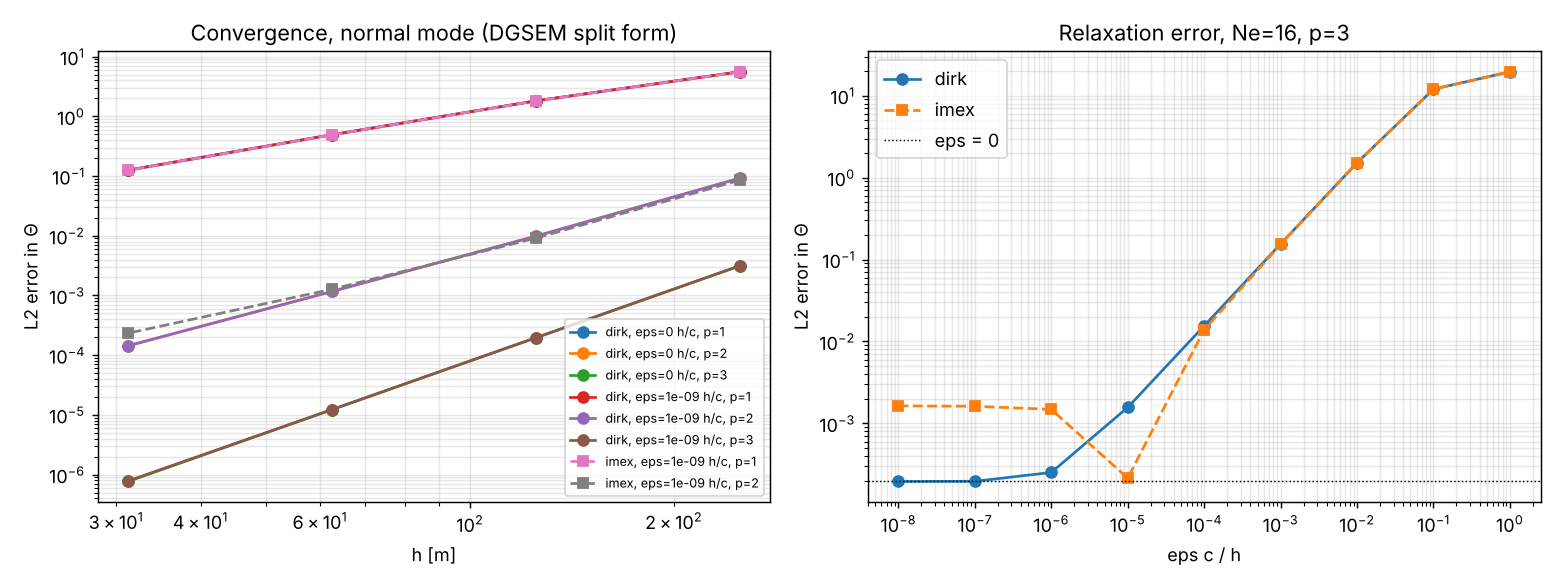
\includegraphics[width=\textwidth]{theta_convergence.png}
\caption{Left: convergence. Right: relaxation error versus $\varepsilon c/h$.}
\end{figure}}{}
\IfFileExists{theta_wall_demo.png}{%
\begin{figure}[h]\centering
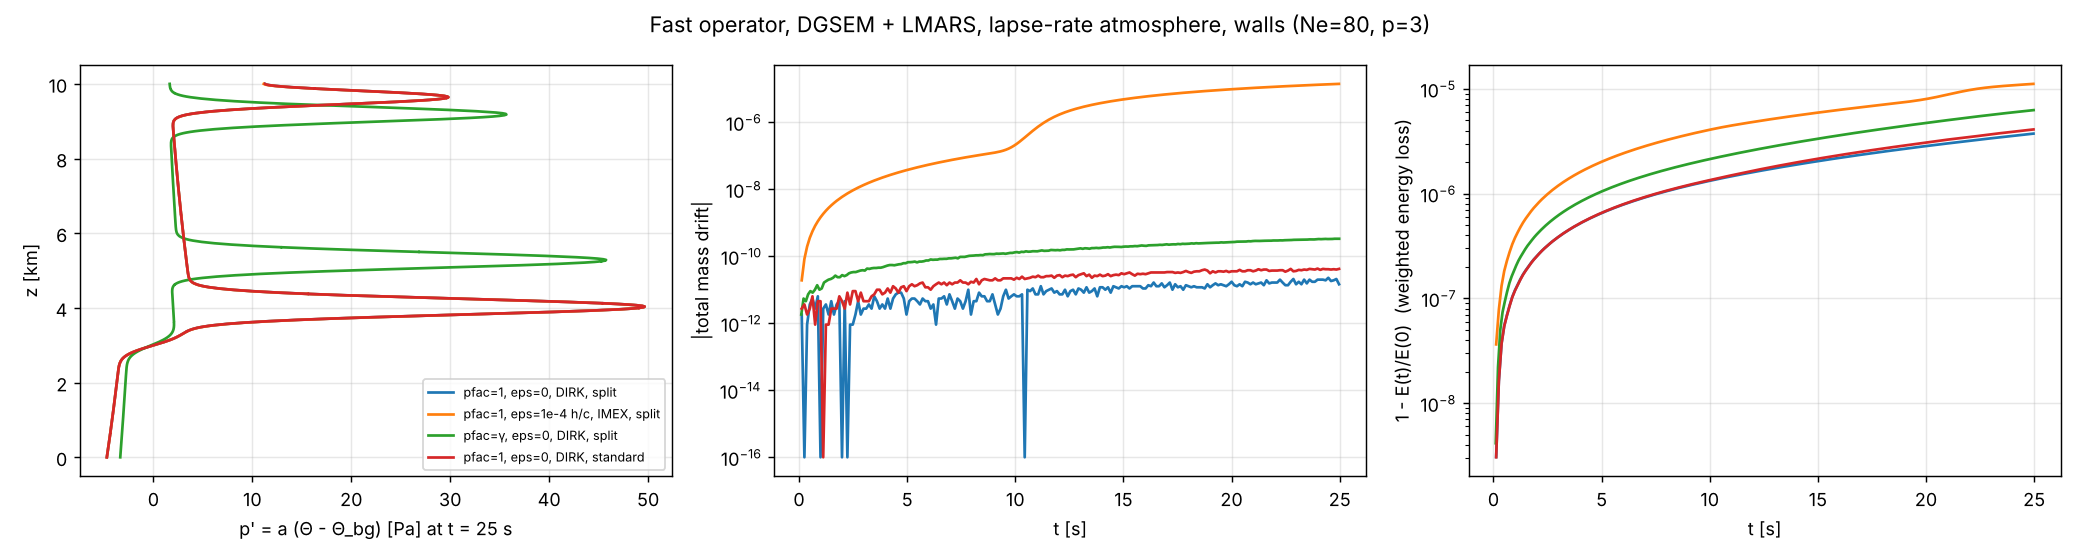
\includegraphics[width=\textwidth]{theta_wall_demo.png}
\caption{Pulse at $t=25$\,s (left), mass drift (middle), and loss of weighted energy
$1-E/E_0$ (right).}
\end{figure}}{}

%=====================================================================
\section{Code}
%=====================================================================
\begin{tabular}{ll}
\texttt{hdg\_relax\_theta.py} & Python solver (NumPy/SciPy)\\
\texttt{run\_tests\_theta.py} & Python tests and plots\\
\texttt{julia/HDGRelaxTheta.jl} & Julia module (standard library only)\\
\texttt{julia/run\_tests\_theta.jl} & Julia tests, writes CSV files\\
\end{tabular}

\subsection*{Data layout}
Nodal value $(e,r,i)$ (element, variable $\rho,m,\Theta$, GLL node from bottom to top) is stored
at $((e-1)\cdot3+(r-1))(p+1)+i$ in Julia (1-based) and at $(3e+r)(p+1)+i$ in Python (0-based).
Trace $(f,r)$ is stored at $3(f-1)+r$ (Julia) or $3f+r$ (Python). The state is $\bm U=(\q,\qh)$.

\subsection*{Usage (Julia)}
\begin{lstlisting}
include("HDGRelaxTheta.jl"); using .HDGRelaxTheta
atm = Atmosphere(T0 = 288.0, Γ = 0.0065)
fr  = frozen_from_atmosphere(atm; pfac = 1.0)      # or FrozenState(pi_fun, theta_fun; ...)
s   = HDGRelaxTh(80, 3, 0.0, 1.0e4, fr; bc = :wall, eps = 0.0, form = :split)
q   = balanced_state(s, z -> atm_Theta(atm, z))     # discrete hydrostatic state
F   = zeros(s.nq)                                   # slow tendency (split-explicit)
U   = run!(s, initial_state(s, q), 0.05, 100; method = :imex, F_slow = F)
z, Q = evaluate(s, U[1:s.nq])                       # Q[1,:]=ρ, Q[2,:]=ρw, Q[3,:]=ρθ
\end{lstlisting}
Python:
\begin{lstlisting}
s = HDGRelaxTheta(Ne, p, zmin, zmax, FrozenState.from_atmosphere(atm, pfac),
                  bc="wall", eps=0.0, form="split")
U = s.run(U0, dt, n, method="imex", F_slow=F)
\end{lstlisting}
To freeze coefficients from a DG slow state, pass functions that return its continuous nodal
values of $\bar p/\bar\Theta$ and $\thb$. The energy weight $\varphi$ is built internally.

\begin{thebibliography}{9}
\bibitem{chen2013} X.~Chen, N.~Andronova, B.~van Leer, J.~E.~Penner, J.~P.~Boyd, C.~Jablonowski,
S.-J.~Lin, A control-volume model of the compressible Euler equations with a vertical Lagrangian
coordinate, \emph{Mon.\ Wea.\ Rev.} 141 (2013) 2526--2544.
\bibitem{gassner2013} G.~J.~Gassner, A skew-symmetric discontinuous Galerkin spectral element
discretization and its relation to SBP-SAT finite difference methods, \emph{SIAM J.\ Sci.\
Comput.} 35 (2013) A1233--A1253.
\bibitem{kopriva} D.~A.~Kopriva, \emph{Implementing Spectral Methods for Partial Differential
Equations}, Springer, 2009.
\bibitem{ars} U.~M.~Ascher, S.~J.~Ruuth, R.~J.~Spiteri, Implicit-explicit Runge--Kutta methods for
time-dependent partial differential equations, \emph{Appl.\ Numer.\ Math.} 25 (1997) 151--167.
\bibitem{hairer} E.~Hairer, G.~Wanner, \emph{Solving Ordinary Differential Equations II: Stiff and
Differential-Algebraic Problems}, 2nd ed., Springer, 1996.
\bibitem{wicker2002} L.~J.~Wicker, W.~C.~Skamarock, Time-splitting methods for elastic models using
forward time schemes, \emph{Mon.\ Wea.\ Rev.} 130 (2002) 2088--2097.
\end{thebibliography}
\end{document}
